\documentclass{article}
\usepackage{graphicx} % Required for inserting images
\usepackage{babel}[polish]
\usepackage{polski}
\usepackage{float}
\usepackage{adjustbox}
\usepackage{subfig}
\usepackage{booktabs}
\usepackage{siunitx}
\usepackage[a4paper,top=2cm,bottom=2cm,left=3cm,right=3cm,marginparwidth=1.75cm]{geometry}
\usepackage{tikz}
\usepackage{pgfplots}
\usepackage{pgfplotstable}
\usepackage{amsmath}
\usepackage{filecontents}
\usepackage{wrapfig}
\usepackage{svg}
\usepackage{tabularx}
\usepackage{array}
\newcolumntype{Y}{>{\centering\arraybackslash}X}
\usepackage{xcolor,colortbl}
\usepackage{pdfpages}

\pgfplotsset{compat=newest}
\usepgfplotslibrary{external}
\tikzexternalize[prefix=tikz/]

\title{ELA2 - Projekt}
\author{Piotr Pokornowski 325061}
\date{\today}

%\pgfplotstableread[col sep=semicolon]{figures/digital/output.csv}\digital

\pgfplotsset{select coords between index/.style 2 args={
            x filter/.code={
                    \ifnum\coordindex<#1\def\pgfmathresult{}\fi
                    \ifnum\coordindex>#2\def\pgfmathresult{}\fi
                }
        }}

\begin{document}

\maketitle

\newpage

\section{Sekcja cyfrowa}
\subsection{Opis układu}
Zaprojektowana przetwornica obniża napięcie z \SI{10}{\V} do \SI{5}{\V} i działa dla prądu maksymalnego \SI{5}{\A}. Jej zadaniem jest zasilanie cyfrowej sekcji układu, z tego powodu minimalizacja tętnień była celem drugorzędnym, a priorytetem stało się uzyskanie jak największej sprawności \textemdash \ dla maksymalnego obciążenia prądem \SI{5}{\A} udało się uzyskać sprawność na poziomie $\sim \SI{94.3}{\percent}$.

\begin{figure}[H]
    \centering
    \begin{adjustbox}{width=1.1\textwidth,center}
        \subfloat[Schemat układu]{
            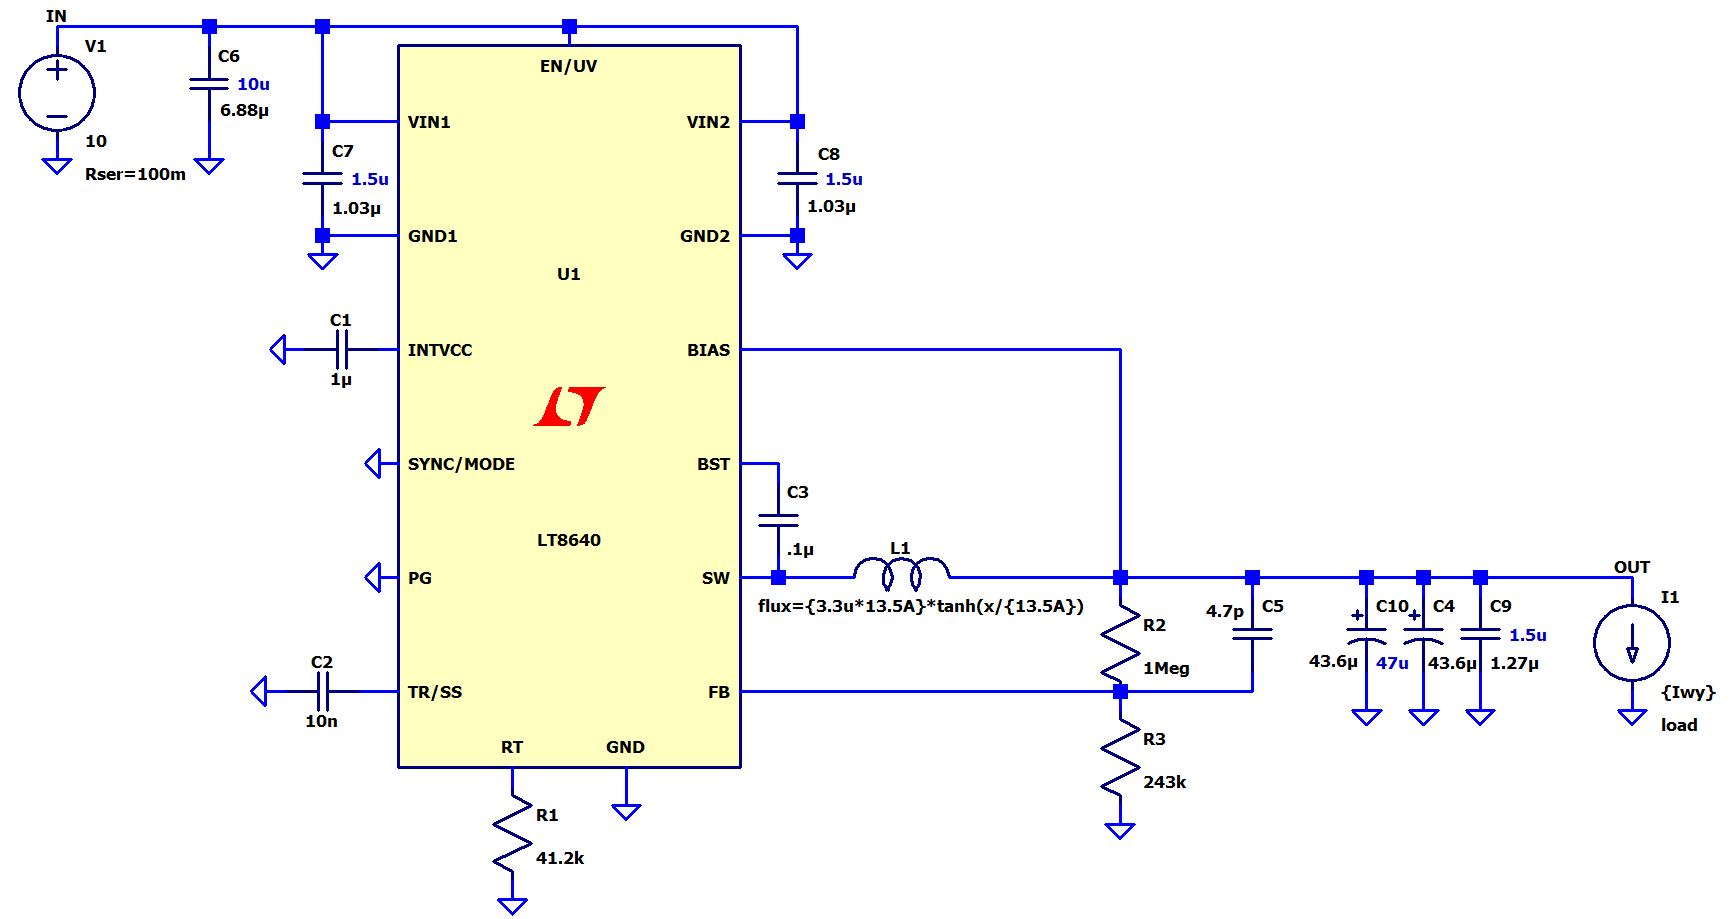
\includegraphics[width=\textwidth]{./figures/digital/digital.png}
            \label{fig:subfig1}
        }
        \qquad
        \subfloat[Przebiegi czasowe prądu i napięcia na wyjściu układu]{

        }
    \end{adjustbox}
\end{figure}

\subsection{Wybór elementów}
Wykorzystany układ LT8640 został wybrany, ponieważ spełniał wymagania projektowe oraz był dostępny w dużych ilościach wśród dostawców, dodatkowo Analog Devices sugeruje go jako jeden z układów do wykorzystania przy nowych projektach.\\
Cewka została dobrana zgodnie ze wzorem $L = \frac{V_{OUT} + V_{SW(BOT)}}{f_{SW}} \approx \SI{3.6}{\micro\H}$ dostępnym w nocie katalogowej. W układzie znalazła się więc najbliższa z szeregu cewka o wartości \SI{3.3}{\micro\H}, podobna cewka o takiej samej wartości jest używana w przykładowym układzie producenta.\\
Kondensatory zostały dobrane zgodnie z zaleceniami producenta układu, jednocześnie biorąc pod uwagę spadek pojemności. Wszystkie użyte kondensatory to kondensatory MLCC, z wyjątkiem dwóch dużych kondensatorów wyjściowych. Zamiast MLCC użyte są tam aluminiowe kondensatory elektrolityczne, co pozwoliło na znaczną redukcję kosztów przy zachowaniu dobrych parametrów \textemdash \ wykorzystanie w tym miejscu trudno dostępnych kondensatorów ceramicznych o pojemności \SI{47}{\micro\F} byłoby nieopłacalne, gdyż kosztowały one więcej niż cała reszta elementów w układzie. Dokładne informacje o elementach znajdują się w pliku BOM.

\end{document}
